\documentclass{article}
\usepackage{gensymb}
\usepackage{amsmath}  % improve math presentation
\usepackage{graphicx} % takes care of graphic including machinery
\usepackage{wrapfig}
\usepackage{xcolor}
\usepackage{setspace}
\usepackage[final]{hyperref} % adds hyper links inside the generated pdf file
\hypersetup{
	colorlinks=true,       % false: boxed links; true: colored links
	linkcolor=blue,        % color of internal links
	citecolor=blue,        % color of links to bibliography
	filecolor=magenta,     % color of file links
	urlcolor=blue         
}
%++++++++++++++++++++++++++++++++++++++++
\graphicspath{{./figs/}}
%\usepackage[round]{natbib}

\newcommand{\caution}{
	\textbf{\textit{ \textcolor{red}{Use caution.} }}
}

\title{Pressure Vessel Setup Workflow}
\author{Clay Wood}
\date{}

\begin{document}
	
\maketitle

\tableofcontents

\section{a section}
something something something. 

%\centering{{\Large \textbf{Pressure Vessel Setup Workflow -- Draft}}}
%{\Large \textbf{Pressure Vessel Setup Workflow -- Draft}}
%\vspace{-0.1 in}
%\bigskip
%\hrule

%\bigskip
\begin{flushleft}
\textbf{Inserting Vessel into Biax:}
	\begin{itemize}
		\item \textit{Move both pistons to minimum position.}
		\item Disconnect and remove DCDTs,  load cells, and limit switches.
		\item Maneuver Vessel cart in front of biax.
		\item Rotate Vessel such that the bottom/top face horizontal piston, then carefully slide it into Biax.
		\item Flip Vessel upright. 2 persons required to act as fulcrum and lever. \caution
		\item Insert metal spacer blocks ($ \times $ 4) and shims ($\times $ 3) and align Vessel.
		\item Reconnect and install all DCDTs, load cells, and limit switches, \textit{except for vertical DCDT}.
	\end{itemize}

\textbf{Preparing Vessel for Confining Fluid:}
	\begin{itemize}
		\item \textit{Inspect all fluid port connections (top \& internal) for damage (threading) -- replace if necessary}.
		\item Insert horizontal and vertical piston extensions (pucks) through respective orifices using nose cone. 
		\item Insert appropriate corner and spacing blocks for respective SDS or DDS configuration. 
		\item Put in sample, align, and connect to internal fluid ports. Everything must be properly aligned to prevent stress concentrations. Some setups include an internal DCDT or other additional measurement devices.
		\item \textit{Remove old excess vacuum grease and oil from both door O-rings and inspect for damage -- replace if necessary. }
		\item Thoroughly clean o-ring indents on Vessel. Uniformly coat o-rings with vacuum grease (surface should feel tacky) and install. 
		\item \textbf{Securing Vessel Doors:}
		\begin{itemize}
			\item Apply a small horizontal stress ($\approx  1$ MPa) on sample to prevent rotation of Vesssel. 
			\item Carry \textbf{\textit{back}} door ($P_c$ and ultrasonic connections) to back of Biax and rest between base and horizontal load frame. DDS configuration: connect ultrasonic cables now. Lift door into place and gently align into opening.  \caution When properly aligned, the door can be gently pushed into Vessel.
			\item Process is similar for \textbf{\textit{front}} door, except for ultrasonic connections. \caution
			\item Put bolts (w/ washer) in all door holes and tighten with pneumatic screw driver.  
			\item Use large wrench to completely tighten all bolts in 2 rounds. Do not tighten in a circular pattern, see Figure \ref{fig:bolt_tight} for suggested tightening scheme.
			 The wrench should make a clicking sound (indicating tightness) for all bolts in second round. 
		\end{itemize}
		\item Connect and tighten $P_c$ line and tube from oil tank into back door. 
		\item Insert and connect vertical DCDT.
		\item Connect ultrasonic cables from back of vessel to Verasonics.
	\end{itemize}
		
\textbf{Saturating sample:}
	\begin{itemize}
		\item Increase stresses in this order:  $\sigma_n $  and then $P_c $. \textcolor{red}{Rule of thumb: $\sigma_n -  P_c \approx 1$ MPa.}
		\item Connect inlet fluid line from intensifier to top of Vessel and then pressurize.\\ 
		\textbf{\textcolor{red}{Always make sure $\sigma_n >  P_c  > Pp$ .}}\\
		\textcolor{blue}{\textbf{\textit{Note:}} \textit{The stresses, pressures should be optimized to decrease saturation time, but not damage/perturb porous media.} }
		\item Samples with very low permeability may require a vacuum pump to be connect to downstream port at top of vessel, to assist with saturation. 
		\item After pushing through the volume of the intensifier ($\times 2$), then check if sample has been saturated. 
		\item While there is $ Pp_{inlet} $, plug/close valve at downstream and monitor the inlet intensifier displacement rate. If it reaches a steady-state $\approx 0$, and the $ P_c $ is also $\approx 0$, then it unlikely for water to be infiltrating the porous media. 
		\item If $ Pp_{inlet} > 0$, then the sample may not be saturated. 
		\item If  $ P_c \gg 0$ \& no oil is leaking from Vessel exterior, then there may be oil infiltration into the sample. 
	\end{itemize}
\end{flushleft}


\section{something}

\begin{figure}
%	\centering
	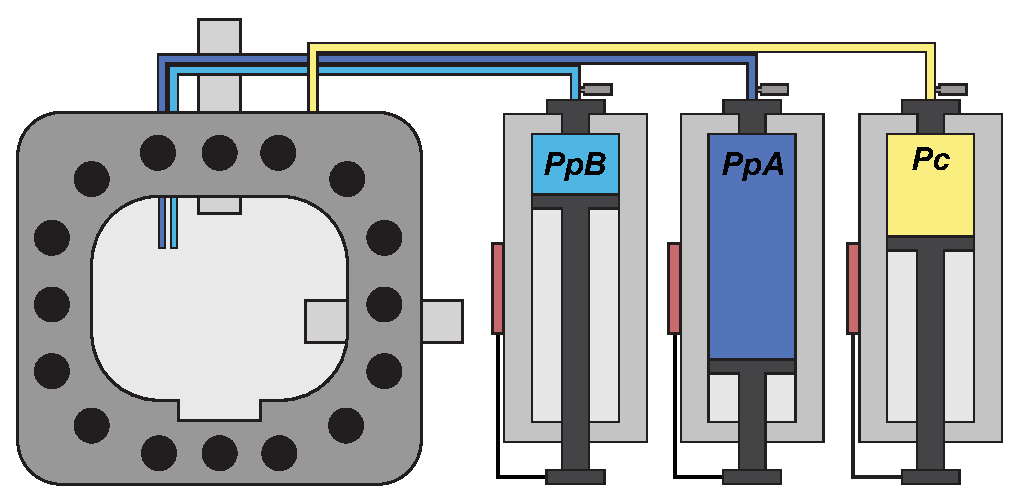
\includegraphics[scale=1]{vessel_config.eps}
	\caption[]{Pressure vessel and pressure intensifiers, $P_pA $, $P_pB $, and $P_c $. The back door has ports to fill from the confining oil reservoir and to pressurize from the $  P_c $ intensifier, and has the availability for connecting to internal acoustics.}
	\label{fig:vessel_config}
\end{figure}

\begin{figure}
	\centering
	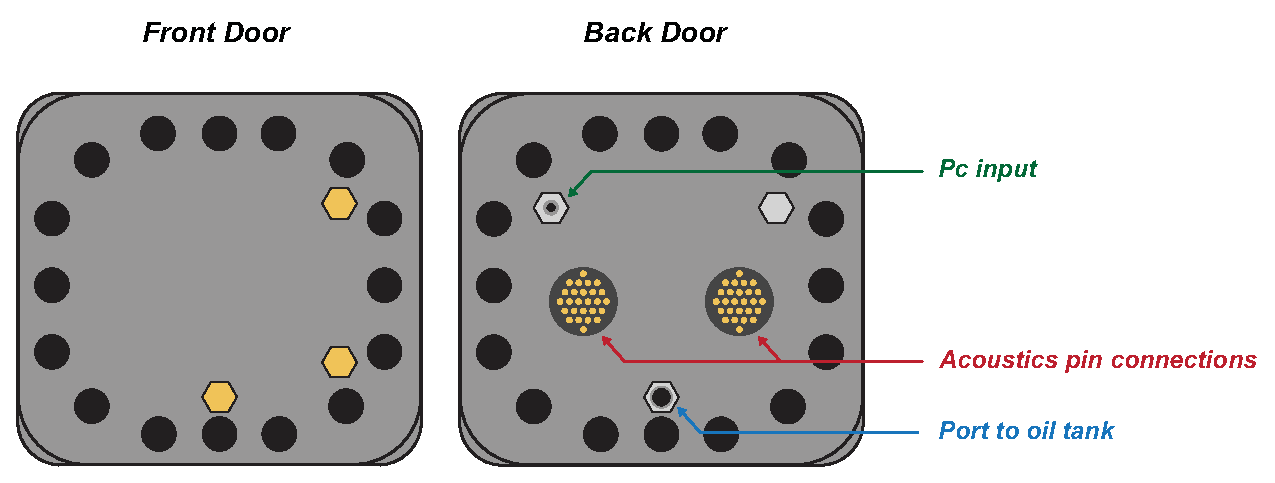
\includegraphics[scale=1]{vessel_doors.eps}
	\caption[]{Vessel door schematic. The back door has ports to fill from the confining oil reservoir and to pressurize from the $  P_c $ intensifier, and has the availability for connecting to internal acoustics.}
	\label{fig:doors}
\end{figure}

%\clearpage

\begin{figure}
	\centering
	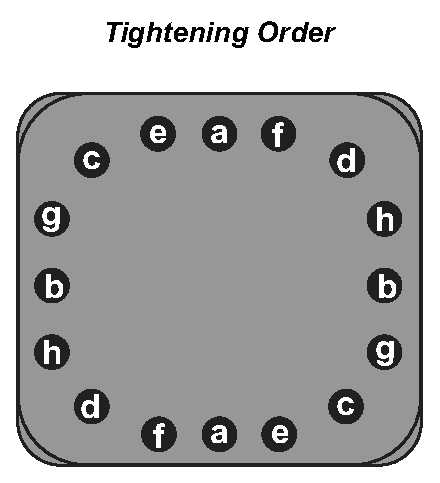
\includegraphics[scale=1]{vessel_door_tighten.eps}
	\caption[]{Suggested order for tightening bolts on vessel doors. Proceed in alphabetical order, opposite pairs, to avoid a circular pattern.}
	\label{fig:bolt_tight}
\end{figure}

\end{document}